\section{
    Effect of uniform relative motions on the Rheology at finite Reynolds number. 
    }
\label{sec:particle_def}


Preceding studies have intended to model the rheology of dilute emulsion of neutrally buoyant deformable droplets, in stokes regime 
\citep{rallison1984deformation,lhuillier1987phenomenology}.
More recently, researchers have been trying to include inertial effects in these models \citep{raja2010inertial,mwasame2018macroscopic}. 
However, these studies have been conducted with the objective of determining the response to the mean shearing motion of a neutrally buoyant suspension on the stress, i.e. they study the mean stress $\bm{\sigma}$ in terms of the imposed flow gradient $\textbf{E}_f$ for a given microstructure. 
To the knowledge of the author all preceding study disregards the impact of relative motion, that we denote $\textbf{u}_{fp} = \textbf{u}_f - \textbf{u}_p$, on the suspension rheology.


In this section, we make use of the \textit{hybrid model} derived in the preceding sections to demonstrate what is the effect of uniform phase relative motion on the rheology at finite Reynolds number. 
As this problem is rather complicated we first use some simplifying hypotheses. 
We start by considering only uniform relative motion. 
Indeed, as the purpose is to point out the effect of the relative translational motions on the stress, we consider that there is no mean shear within the emulsion, i.e. $\textbf{E}_f = 0$. 
As discussed in the preceding section we consider that the droplet shape relaxes instantaneously with the ambient fluid motion, in other words we consider that the deformations of the drops are in a quasi-steady state regime with the solicitation of the flow. 
Finally, as stated in the beginning of this chapter we only focus on small deformations.  



To introduce the problem we first present a way to compute analytically the droplet deformation in terms of its relative motion with the carrier phase. 
Indeed, it is shown with the help of the reciprocal theorem that the closure term of \ref{eq:dev} can be obtained at $\mathcal{O}(Re \phi)$.
Doing so we obtain an explicit formula for the droplet deformation. 
We deduce from this application that at a finite Reynolds number, the first moment of the hydrodynamic forces cause the droplet deformation and acts as a source term inside the mean carrier fluid stress. 
Therefore, in the second step, we expose a closed formulation of the bulk stress of the carrier fluid phase. 


The particle averaged linear momentum and mass conservation, can be obtained carrying the same procedure as in \ref{chap:daniel1} and yield the same as for non-deformable particles. 
Only the closure terms of the latter equations will be influenced by considering the drop shape and orientation.
The same comments can be made regarding the carrier phase equations. 
This implies that the equations used in \ref{chap:daniel1} are still valid upon having the right closure terms. 
Consequently, for a mono-disperse suspension, these equations provide an equation for the mean particle phase velocity $\textbf{u}_p$ fluid velocity $\textbf{u}_f$ and particle volume fraction $\phi_f$ or $\phi_d$. 
Thus, in the next paragraphs, we will consider these variables as known variables. 

\subsection{Determination of the averaged particle shape}

In \ref{chap:deformable} we have seen that in the quasi-steady state regime the rate of strain equation, i.e. the equation for $\textbf{E}_\alpha$, reduces directly to an equation for the particle shape $\bm\chi_p$. 
Thus, we will use \ref{chap:deformable} to compute the averaged particle shape. 
Applying the average operator on \ref{eq:steady} yields,
\begin{equation}
    \bm\chi_{p}
    = 
    \frac{5}{4}Ca \left[
        (\textbf{F}_p^h )^*
        + \zeta Re (\textbf{F}_p^{vv})^*
        +    \lambda (\textbf{F}_p^{\sigma})^*
    \right],
    \label{eq:steady_state_avg}
\end{equation}
where we introduced, $n_p \textbf{F}_p^h = \pavg{\textbf{F}_\alpha^h}$ and so on. 
Thus, in this regime, one might be able to compute the instantaneous averaged shape of the particle upon the knowledge of the mean surface stress distribution, $\textbf{F}_p^h$, the mean particle's internal shear stress tensor, $\textbf{F}_p^{\sigma}$, and finally, the mean particle internal inertial contribution $\textbf{F}_p^{vv}$. 

As the purpose of this section is to determine the effect of relative motion on the shape of the particles, we will consider only the closures that are functions of $\textbf{u}_{pf}$, which is the relative phase velocity. 

\subsubsection{Discussion on the closure problem}   

However, to broaden our understanding, we first propose to discus what form the right-hand side of \ref{eq:steady_state_avg} may take in the simplest scenario. 
Only for this subsection we consider a mean shear rate $\textbf{E}_f$ since it is useful for the subsequent discussion. 

Let us first discuss the term $\textbf{F}^{vv}$. 
It is clear that a complete closure for this term taking into account all parameters at hand is impossible. 
Nevertheless, as shown in \ref{ap:reciprocal} we may already compute this term assuming only the translation of a spherical droplet in a pure linear stokes flow. 
As this term is inertial by nature, its computation from the Stokes flow solution just gives us the first order in $Re$ accurate term.
Thus, for $Re \zeta < 1$, $Ca = 0$ and $\phi = 0$ we may write,
\begin{multline}
    n_p m_p U^2 (\textbf{F}^{vv}_p)^*
    % &= 
    % \intO{\rho_d [\textbf{v}_d^0  \textbf{v}_d^0  - \frac{1}{3}\rho_d (\textbf{v}_d^0 \cdot \textbf{v}_d^0)\bm\delta]}\\
    = 
    \frac{\rho_d \phi_d}{20(\lambda +1 )^2}
    \left[
        \textbf{u}_{p f}\textbf{u}_{p f} 
    -\frac{1}{3} (\textbf{u}_{p f}\cdot \textbf{u}_{p f})\bm\delta
    % + 7\pavg{\textbf{u}_\alpha'\textbf{u}_\alpha'}/n_p 
    % + 2k_p \bm\delta
    \right]\\
    + \frac{\rho_d \phi_d a^2}{21 (\lambda + 1)^2}[\textbf{E}_f\cdot \textbf{E}_f - \frac{1}{3}(\textbf{E}:\textbf{E})\bm\delta]
    + \mathcal{O}((Re\zeta)^2,Ca, \phi)
    \label{eq:vv_closure}
\end{multline}
where $U = |\textbf{u}_{pf}|$ is the velocity scale. 
This closure is valid solely for spherical particles at first order in $Re$. 
Thus, as soon as the particle deforms an additional correction must be provided to account for this deformation. 
Note that these corrections can be obtained at low but finite capillary number $Ca$, from \citet{leal2007advanced} for a droplet immersed in pure linear flows, and \citet{taylor1964deformation} for a droplet in relative translation. 
Indeed, these authors provide the detailed velocity fields of such cases. 
Anyhow, we would like to point out that due to the presence of $\textbf{u}_{p f}$ in \ref{eq:vv_closure} the internal droplets motions, $\textbf{v}_d^0$, induce a coupling between the droplets translational motion $\textbf{u}_\alpha$ and deformation $\bm\chi_\alpha$ through \ref{eq:dev_dim}. 
As could be expected, the fluid phase shear rate $\textbf{E}_f$ also induces an internal motion (see \ref{fig:flowlines}), which when accounting for the particle inertia plays a role in the dynamical shape balance.  
To conclude, note that $\textbf{F}^{vv}$ is the only reason why the density ratio $\zeta$ comes into play when computing the steady-state shape of a droplet (for example see \citet{taylor1964deformation}). 

The internal particle shear rate forcing term $\textbf{F}^\sigma$, also plays an important role in the shape dynamics. 
Applying the previous reasoning we obtain a first glimpse of the functional form of this term. 
Indeed, from \ref{ap:reciprocal} we found that, 
\begin{equation*}
    \frac{n_p v_p  \mu_d U}{a}(\textbf{F}_p^{\sigma})^*
    % = - \mu_d \intS{(\textbf{n}_i \textbf{v}_{d,j}^0 + \textbf{n}_j \textbf{v}_{d,i}^0)}
    = \mu_d \phi \frac{ 2 }{\lambda+1}
    \textbf{E}_f
    + \mathcal{O}(Re,Ca,\phi). 
\end{equation*}
In this situation note the absence of $\textbf{u}_{fp}$ in the expression.
This is because the translation of a droplet in stokes flow does not alter the shape of the droplets. 
Nevertheless, at $\mathcal{O}(Re^2)$ it is reasonable to expect the emergence of terms proportional to $\textbf{u}_{fp}$ in the expression.
Approximately the same treatment can be adopted for the external stress contribution $\textbf{F}^h$. 
Indeed, it is found that, 
\begin{equation}
    % \pavg{\intS{\textbf{r}\bm{\sigma}_f^0 \cdot \textbf{n}_d}} 
    \frac{n_p v_p \mu_f U}{a}
    (\textbf{F}^h_p)^*
    = 
    \frac{3}{5}\mu_f \phi_d \left(\frac{2+5\lambda}{1+\lambda}\right)
    \textbf{E}_f
    + \mathcal{O}(Re,Ca,\phi).
    \label{eq:closure_stress}
\end{equation}
Again at the next order in $Re$ it is likely that the translation of the droplet might contribute to this term. 
Indicating a coupling between deformation and relative translation. 
Nevertheless, under this form, the closure problem is incomplete as \ref{eq:dev} requires to compute the closure term with an accuracy of $\mathcal{O}(Ca)$ at least. 
Note that in \citet{raja2010inertial} they give the next order in $Re$ for this term.


Overall, we have shown that these closure terms can indeed be expressed as a combination of particles and carrier fluid properties.
Particularly, we demonstrated that there is an explicit link between deformation and translational velocity of the particle at finite $Re$, through the term $\textbf{F}^{vv}_p$. 
% Overall, we have shown that these closures could be expressed based on the singularity solution of stokes flows. 
Thus, it is clear that the relative velocity plays a role only at finite Reynolds numbers. 
Indeed, at $Re = 0$ only the mean fluid shear rate $\textbf{E}_f$ is present in the source terms, $\textbf{F}^h_p$ and $\textbf{F}_p^{\sigma}$. 
Therefore, as our objective is to determine the effect of relative motion on the shape of the particle, we decided to compute the closure terms at $\mathcal{O}(Re)$. 
Indeed, at finite $Re$ it will eventually make appear the relation of these closures with the relative motion $\textbf{u}_{pf}$. 


\subsubsection{Determination of the closure terms at first order in $Re$}

To determine the $\mathcal{O}(Re)$ correction of $\textbf{F}_p$ the closure terms of we first expand the RHS of \ref{eq:steady_state_avg} in at Taylor expansion about $Re = 0$. 
We obtain the following relation, 
\begin{align*}
    (\textbf{F}_p)^*(Re)
    = 
    \textbf{F}_p^{(0)}
    + Re\textbf{F}_p^{(1)}
    + \ldots 
    = 
    [(\textbf{F}^h_p)^{(0)}+\lambda (\textbf{F}^\sigma_p)^{(0)}]
    + Re[(\textbf{F}^h_p)^{(1)}+\lambda (\textbf{F}^\sigma_p)^{(1)}+\zeta (\textbf{F}^{vv}_p)^{(0)}]
    + \ldots 
\end{align*}
where the terms with superscript $^{(0)}$ correspond to the adequate stokes flow solution, and the terms with $^{(1)}$, to the first inertial correction solution. 
It is interesting to note that to be accurate at first order in $Re$ we only need to compute the term $(\textbf{F}^{vv}_p)^{(0)}$.
In other words, this term is the integral of the particle's internal velocity for a translating sphere in stokes flow.  
Indeed, as we are interested only in the particle relative translation we can already obtain this term from \ref{eq:vv_closure}, which reads 
\begin{equation}
    (\textbf{F}^{vv}_p)^{(0)}
    % &= 
    % \intO{\rho_d [\textbf{v}_d^0  \textbf{v}_d^0  - \frac{1}{3}\rho_d (\textbf{v}_d^0 \cdot \textbf{v}_d^0)\bm\delta]}\\
    = \frac{1}{20(\lambda +1 )^2}
        [\textbf{u}_{p f}^*\textbf{u}_{p f}^* 
    -\frac{1}{3} (\textbf{u}_{p f}^*\cdot \textbf{u}_{p f}^*)\bm\delta]. 
    % + 7\pavg{\textbf{u}_\alpha'\textbf{u}_\alpha'}/n_p 
    % + 2k_p \bm\delta
    \label{eq:closure_vv}
\end{equation}
Where we introduced $\textbf{u}_{pf}^* = \textbf{u}_{pf} / U $. 
Regarding the term $(\textbf{F}^h_p)^{(1)}$ and $\lambda (\textbf{F}^\sigma_p)^{(1)}$, the calculation becomes more complicated since it requires the solution at first order accuracy in $Re$ for the fields $\bm\sigma_f^{(1)}$ and $\textbf{u}_f^{(1)}$. 

In \ref{ap:reciprocal} we demonstrate how to compute $(\textbf{F}^h_p)^{(1)}$ and $\lambda (\textbf{F}^\sigma_p)^{(1)}$. 
The method is based on the reciprocal theorem, following the strategy used in \citet{stone2001inertial,masoud2019reciprocal} for solid particles. 
% for finite $Re$ and is not limited to the context presented here.
Specifically in \ref{ap:reciprocal} we show how to compute the first order correction in $\mathcal{O}(Re)$ of any moment of hydrodynamic forces on the surface of a spherical droplet immersed in an arbitrary flow. 
While this general derivation can be of interest in other problems, we focus specifically on deriving the closure terms present in \ref{eq:vv_closure} under the assumption of uniform relative motion between particles and carrier fluid. 
% We show that the computation of $(\textbf{F}^h_p)^{(1)}$, independently of $\lambda (\textbf{F}^\sigma_p)^{(1)}$ was not possible, however we could demonstrate  how to compute the sum of these terms. 


We show with the reciprocal theorem that the first-order correction of the internal particle stresses is identically null, meaning $(\textbf{F}^\sigma_p)^{(1)} = 0$. 
Regarding the traceless and symmetric part of the first moment of hydrodynamic forces, we obtained, 
\begin{align}
    (\textbf{F}^h_p)^{(1)}  
    % + \lambda (\textbf{F}^\sigma_p)^{(1)}
    &=
    C_1 
    [
        \textbf{u}_{pf}^*\textbf{u}_{pf}^* - \frac{1}{3}(\textbf{u}_{pf}^*\cdot \textbf{u}_{pf}^*)\bm\delta 
    ]\\
    C_1 &=
    % \frac{345 \lambda^{3} + 928 \lambda^{2} + 856 \lambda + 272}{320 \left(\lambda + 1\right)^{3}}
    % + \frac{\zeta \left(12 \lambda + 13\right)}{20 \left(\lambda + 1\right)^{2}}
    - \frac{63 \lambda^{3} + 150 \lambda^{2} + 112 \lambda + 28}{80 \left(\lambda + 1\right)^{3}}
    % \intS{\textbf{u}_f^{(1)}\cdot  \hat{\bm\sigma}_f \cdot \textbf{n}}
    % \intOf{\textbf{u}_f^{(0)}\cdot ( \div \hat{\bm\sigma}_f)}
    \label{eq:closure_sigma_e}
\end{align}
% This, proves indirectly that the Stresslet on a drop in translation is not null at finite $Re$.
% where $v_p$ is the averaged volume of the particles, here $v_p = 4/3 \pi a^3$.  
Thus, a translating droplet experiences a non-zero first moment of the hydrodynamic forces due to the inertial effects of the surrounding fluid. This result indicates that the stress distribution over the surface of the particle is unbalanced, which, as we will see, leads to particle deformation.
This contrasts with the Stokes flow case, where the hydrodynamic stress is balanced, as we've observed that $(\textbf{F}^h_p)^{(0)} = 0$ when considering only relative translation.  
% Note that this derivation is based on spherical droplets' solution. 
% Thus, they are only accurate at zeroth order in  $\mathcal{O}(|\bm\chi|)$. 


Using \ref{eq:closure_vv} and \ref{eq:closure_sigma_e} in  \ref{eq:steady_state_avg}, the deformation of the droplets can be estimated at $\mathcal{O}(Re,Ca,\phi)$ and yields, 
\begin{align}
    (\bm\chi_{p})_{ij}
    &= 
    \frac{5}{4}We \left[
        (\textbf{F}_p^h )_{ij}^{(1)}
        + \lambda (\textbf{F}_p^{\sigma})_{ij}^{(1)}
        + \zeta (\textbf{F}_p^{vv})_{ij}^{(0)}
    \right]
    \label{eq:deformation_final1}
    \\
    &= We \beta [\textbf{u}_{pf}^*\textbf{u}_{pf}^* - \frac{1}{3}(\textbf{u}_{pf}^*\cdot \textbf{u}_{pf}^*)\bm\delta ]
    + \mathcal{O}(Re^{3/2},\phi,Ca),
    \label{eq:deformation_final}
\end{align}
with, 
\begin{equation}
    \beta = 
    \frac{\zeta}{16 \left(\lambda + 1\right)} 
    % - \frac{63 \lambda^{3} + 150 \lambda^{2} + 112 \lambda + 28}{80 \left(\lambda + 1\right)^{3}}
    - \frac{63 \lambda^{3} + 150 \lambda^{2} + 112 \lambda + 28}{64 \left(\lambda + 1\right)^{3}}
    \label{eq:beta_coef}
\end{equation}
where we have introduced the \textit{Weber} number $We = Re \cdot Ca$. 
Note that the first term of the coefficient $\beta$ obtained here agrees with the deformation derived by \citet{taylor1964deformation}, (noted $\zeta$ in their work), if one account for the two different definitions of the ``deformation'' used in our work and in \citet{taylor1964deformation}, inducing a factor equal to $2$ in front of his coefficient $\zeta$.
However, the second term of \ref{eq:beta_coef} found by \citet{taylor1964deformation}, does not agree exactly.
At this stage, the authors cannot understand the source of this inconsistency between the results.

In \ref{fig:beta} we display the different values that $\beta$ can adopt in terms of $\lambda$ and $\zeta$. 
It is found that $\beta$ is negative for all $\lambda$ when  $\zeta = 0, 1$, which means that the droplet will eventually deform into an oblate spheroid for bubbles and viscous droplets rising in a fluid. 
\begin{figure}[h!]
    \centering
    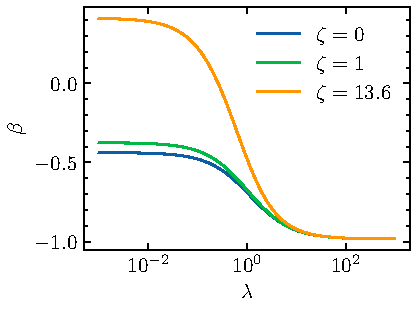
\includegraphics[height=0.25\textwidth]{image/Theory/beta.pdf}
    \caption{Values of the constant $\beta$ in terms of $\lambda$ for multiples values of $\zeta$. 
    $\zeta = 0,1,13.6$ corresponds respectively to, a bubble in water, a drop oil in water and a drop of mercury in water. }
    \label{fig:beta}
\end{figure}
However, when the density ratio of the droplet to that of the carrier fluid is high, for example, when $\zeta = 13.6$ we should expect a prolate spheroidal shape. 
This conclusion aligns with \citet{taylor1964deformation} even if as said the exact value of $\beta$ could not be recovered. 

Let us now discuss the physical implication of the droplets deformation. 
If the droplets deform, this means that the local forces above and below the droplet are stronger than the forces on the sides of the droplets. 
If the droplets experience this distribution of forces on their surfaces, this means that the continuous phase experiences an equal, but opposite in sign distribution of forces from the surface of the droplets. 
Consequently, the average carrier fluid phase stress will be impacted by the non-vanishing value of $\textbf{F}^h_p$ as well. 

\subsection{The continuous phase stress}

In this section, we would like to compare the relative influence of the first moment of the hydrodynamic forces due to relative translating motions, to the other contributions present in the continuous phase equivalent stresses. 
For the comparison to be meaningful $\textbf{F}^h_p$ must be compared to other stresses proportional to $\sim [\textbf{u}_{fp}\textbf{u}_{fp}-\frac{1}{3}(\textbf{u}_{fp}\cdot\textbf{u}_{fp})\bm\delta]$. 
Note that in one dimensional models, for example, the absence of mean shear is inherently assumed, making it essential to discuss the impact of relative translation on the mean stress of the continuous phase. 
Indeed, in such scenarios, terms proportional to the relative motions become the only contributions to the carrier phase stress. 

Now that the motivations are properly stated let us present the expression of the homogeneous averaged continuous phase stress. 
Retaining only the homogeneous terms in \ref{eq:sigma_eq_hybrid} gives, 
\begin{equation}
    \bm{\sigma}^\text{eq}_f = 
    p_f \bm\delta 
    % - 2\mu_f \textbf{e} 
    +\avg{\rho_f\chi_f\textbf{u}_f'\textbf{u}_f'}
    % - \pSavg{\textbf{r}\times(\bm{\sigma}_f^0\cdot \textbf{n}_d)}
    % \\
    - \pSavg{\textbf{r}\bm{\sigma}_f^0\cdot \textbf{n}_d}
    +  \pOavg{(2 \mu_f \textbf{e}_d^0 - p_f\bm\delta)}
    % \\
    % + \div \left[
    %     \frac{1}{2} \pSavg{\textbf{rr}\bm{\sigma}_f^0\cdot \textbf{n}_d}
    %     - 2 \mu_f\pOavg{ \textbf{re}_d^0 }
    %     + \ldots
    % \right]
    \label{eq:sigma_eq_f}
\end{equation} 
Again the mean shear rate $2\mu_f\textbf{e}$, usually present in this expression, does not appear since we are concerned with only relative motion and no macroscopic shear. 
Likewise, the higher order moments of the hydrodynamic force appear under the divergence operator, we therefore neglected them in the attempt to compare only the contribution proportional to $\sim \textbf{u}_{pf}\textbf{u}_{pf}$. 
Under this form it is clear that the mean carrier fluid stress is generated due to the competitive action of the mean continuous phase pressure, the \textit{Reynolds stress} tensor, and the \textit{Stresslet} tensor. 
% As one can see the deformation of the droplets described by $\bm\chi_p$ as well as their rate of strain $\textbf{E}_p$ do not appear explicitly in the equivalent stress. 
% However, that does not mean that they do not play a role in the average stress. 
% Indeed, since the exchange term in \ref{eq:sigma_eq_f} can be substituted using \ref{eq:dt_S} making explicit those quantities witnessing their importance. 
% Nevertheless, as it has been shown, in the steady state regime we obtained algebraic expressions for $\bm\chi_p$ and neglected $\textbf{E}_p$. 
% This means that in this context we may rather directly find a closure for the \textit{Stresslet} and \textit{Reynolds stress} tensor in terms of the particles and carrier fluid properties. 
% Since we only assume relative and uniform motion, closing \ref{eq:sigma_eq_f} means that we must find the relation of these closures with relative mean motion.

In the most general scenario one would solve an equation for $\textbf{u}_p$, $\textbf{u}_f$, $\bm\chi_p$, $\textbf{E}_p$ and, upon having the right closures, he would compute the stress based on this potential expression. 
In the limit of the dilute regime, meaning that we neglect all terms $\sim \mathcal{O}(\phi^2)$ or higher, and only considering relative translational motions, these closures can be determined. 
As we will show in \ref{chap:pseudoturbulence} the \textit{Reynolds stress} tensor can be closed in the steady state homogeneous dilute regime and yields, 
\begin{equation}
    \frac{a \rho_f}{\mu_f U}\avg{\chi_f \textbf{u}_f'\textbf{u}'_f}
    = Re  \phi C^{Re}_1 \left[
        \textbf{u}_{pf}^*
        \textbf{u}_{pf}^*
        -\frac{1}{3}
        (\textbf{u}_{pf}^*
        \cdot\textbf{u}_{pf}^*)\bm\delta
    \right]
    + Re \phi C^{Re}_2 (\textbf{u}_{pf}^*\cdot\textbf{u}_{pf}^*) \bm\delta, 
    \label{eq:Reynolds_stress}
\end{equation}
where, 
\begin{align*}
    C^{Re}_1(\phi,\lambda)
    = 
    % \left[
        \frac{9(2+3\lambda)^2}{80(1+l)^2}\Gamma(1/3) \phi^{-1/3}
        % - (27+82\lambda +62\lambda^2)
    % \right],
    && 
    C^{Re}_2(\phi,\lambda)
    = 
    % \left[
        \frac{(2+3\lambda)^2}{24(1+l)^2}\Gamma(1/3) \phi^{-1/3}
        % - (3+10\lambda +8\lambda^2)
    % \right],
\end{align*}
Where we assumed that the center of mass velocity variance was negligible at  $\phi<0.1$ based on the findings of \ref{chap:pseudoturbulence}. 
Note that the constant $C^{Re}_2$ and $C^{Re}_1$ are still function of $\phi$ due to the non-linear relation of $\avg{\rho_f\chi_f\textbf{u}_f'\textbf{u}'_f}$ with the volume fraction. 
Additionally, we have decomposed the right-hand side terms of \ref{eq:Reynolds_stress}, such that the first term, proportional to $C^{Re}_1$, corresponds to a traceless symmetric tensor, and the second term proportional to $C^{Re}_2$, represents the isotropic contribution.  
Note the constants on the left-hand side of \ref{eq:Reynolds_stress} that are present to obtain a dimensionless result proportional to $Re$. 

The \textit{Stresslet term} has been derived in \ref{ap:reciprocal}. 
As discussed in the later section, it is shown that the zeroth order $Re$ term is identically null. 
However, when first-order inertial effects are considered then we have (see \ref{ap:reciprocal}),
\begin{multline}
    \frac{a}{\mu_f U}\left[
        \pSavg{\textbf{r}\bm{\sigma}_f^0 \cdot \textbf{n}_d}
        - \pOavg{(2 \mu_f \textbf{e}_d^0 - p_f\bm\delta)}
        \right]\\
    =
     \phi Re C_1
    [
        \textbf{u}_{pf}^*\textbf{u}_{pf}^* - \frac{1}{3}(\textbf{u}_{pf}^*\cdot \textbf{u}_{pf}^*)\bm\delta 
    ]
    + Re \phi C_2 (\textbf{u}_{pf}^*\cdot \textbf{u}_{pf}^*) \bm\delta
    % + \phi p_f \bm\delta
    \label{eq:stresslet_trans}
\end{multline} 
with, 
\begin{align}
    C_1  =  -\frac{63 \lambda^{3} + 150 \lambda^{2} + 112 \lambda + 28}{80 \left(\lambda + 1\right)^{3}}
    &&
    C_2  = \frac{3\lambda^2 + 6\lambda + 4}{48(\lambda +1 )^2}
\end{align}
Where the constant $C_1$ is the same as in \ref{eq:closure_sigma_e}, and the constant $C_2$ is computed in  \ref{ap:reciprocal}. 
% We have also assumed that the droplets center of mass velocity variance is negligible at small $\phi$ in this expression. 
In the same way as for the \textit{Reynolds stress} term, we have decomposed the \textit{Stresslet} into an isotropic and symmetric traceless tensor, proportional to $C_2$ and $C_1$, respectively. 
Note that in opposition to \ref{eq:Reynolds_stress}, $C_1$ and $C_2$ are not functions of the volume fraction for the \textit{Stresslet} term. 
As specified in the previous section and demonstrated in \ref{ap:reciprocal}, the last term of \ref{eq:sigma_eq_f} is null even at $\mathcal{O}(Re)$. 


Making use of \ref{eq:Reynolds_stress} and \ref{eq:stresslet_trans} inside \ref{eq:sigma_eq_f} yields the following formula for the carrier fluid averaged stress, 
\begin{multline}
    \frac{a }{\mu_f U}\bm{\sigma}^\text{eq}_f = 
    \left[ p_f + Re \phi  [C^{Re}_2(\phi,\lambda) - C_2(\lambda)](\textbf{u}_{pf}^*\cdot \textbf{u}_{pf}^*) \right]\bm\delta \\
    % - 2\mu_f \textbf{e} 
    % +\avg{\rho_f\chi_f\textbf{u}_f'\textbf{u}_f'} \\
    + Re \phi [C^{Re}_1(\phi,\lambda) - C_1(\lambda)]\left[
            \textbf{u}_{pf}^*\textbf{u}_{pf}^*
            - \frac{1}{3}(\textbf{u}_{pf}^*\cdot \textbf{u}_{pf}^*)\bm\delta
    \right]
    + \mathcal{O}(Re^{3/2},\phi^2, Ca^2 ).
    \label{eq:stress_closed}
\end{multline} 
We note that the terms on the first line on the right-hand side of \ref{eq:stress_closed} correspond to an equivalent pressure term, consisting of:  
(1) The mean hydrostatic pressure of the carrier fluid $p_f$, 
(2) the isotropic contribution from the \textit{Reynolds stress}, and 
(3) the isotropic part of the \textit{Stresslet}, the latter two contribution being proportional to $Re \phi (\textbf{u}_{fp}\cdot \textbf{u}_{fp})$.  
The terms on the second line represent the effective symmetric and traceless part of the carrier phase stress. 
This term arises entirely from the relative motion between the particles and the carrier fluid. 



Overall, at steady state equilibrium and for uniform relative motion the stress is driven by two distinct physical contributions: 
(1) the \textit{Reynolds stress}, also called the particle induced turbulence. 
(2) the \textit{Stresslet} tensor which is also proportional to these two parameters. 
Note that the particle-induced turbulence is well-known term. 
Even though the closure provided here is new, many studies already tackled this issue to model this term in the case of relative motion between phases with solid particles. 
The latter contribution, however, is often taken into account when mean shearing motions are considered, (with \ref{eq:closure_stress} for example), indeed, this term is the cause of the well-known Einstein viscosity. 
However, the value of this term in the presence of relative phase velocity, see \ref{eq:stresslet_trans},  and at $\mathcal{O}(Re)$, have been completely overlooked in the literature. 
Therefore, the presence of this term in the stress constitutive equation \eqref{eq:stress_closed}  is new and seems to have been ignored up to now. 
For these reasons, we now evaluate the relative importance of the \textit{Reynolds stress} often used in this context compared to the \textit{Stresslet} term. 

\begin{figure}
    \centering
    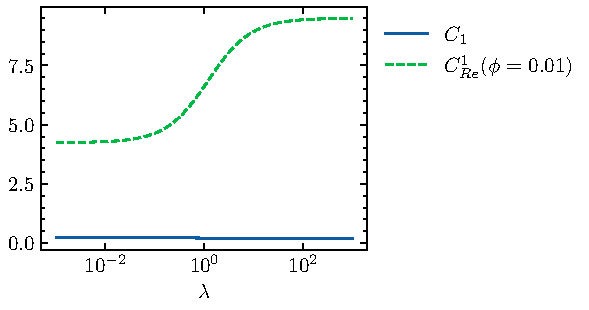
\includegraphics[height=0.25\textwidth]{image/Theory/C1.pdf}
    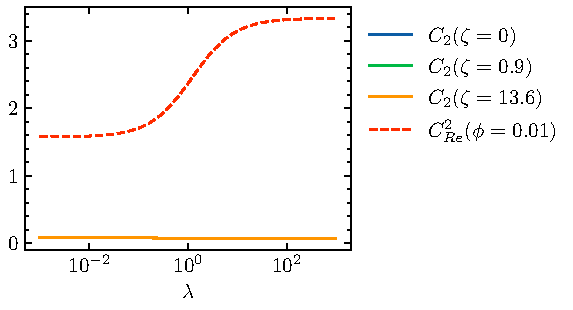
\includegraphics[height=0.25\textwidth]{image/Theory/C2.pdf}
    \caption{
    (solid lines) Values based on \ref{eq:stresslet_trans} of the constant $C_1$ (left)  and $C_2$ (right) in terms of the viscosity ratio $\lambda$.
    (dashed lines) Values based on \ref{eq:Reynolds_stress} of the constant $C_1^{Re}$ (left) and $C_2^{Re}$ (right)  evaluated at $\phi = 0.05$ in terms of the viscosity ratio $\lambda$.
    }
    \label{fig:relative_comparaison}
\end{figure}
Since, $C_1^{Re} \& C_2^{Re} \sim \phi^{-1/3}$ we may already conclude that the $C_1^{Re} \ll C_1$ and $C_2^{Re} \ll C_2$ when $\phi \to 0$. 
This means that for very low volume fractions the \textit{Stresslet} term is completely negligible. 
What about higher volume fractions? 
Since our solution is derived in the dilute limit it seems reasonable to compare the values of the \textit{Reynolds stress} and the \textit{Stresslet} at a maximum value of $\phi = 0.05$. 

% In \ref{fig:relative_comparaison} (right) we compare the vectical contribution of the \textit{Stresslet} and \textit{Reynolds stress} at $\phi =0.05$. 
% By vertical, we mean in the direction of the relative motions. 
% % In this situation we compare the constants $C = \frac{2}{3} C_1 +C_2$ and $C_Re =\frac{2}{3} C^{Re}_1 + C^{Re}_2$ to take in account the total contribution of both stresses in the direction of $\textbf{u}_{fp}$.  
% We can observe that the constant $C_{Re} < C$ regardless of the viscosity ratio $\lambda$. 
% Consequently, the isotropic part of the \textit{Stresslet} due to relative translational motion is less important than the induced pseudo-turbulence.
% However, it still represents a non-negligible part of the stress when $\lambda = 0$ (bubbles in water) where $C^{Re}_2$ is minimum and $C_2$ maximum. 


In \ref{fig:relative_comparaison} (right) we compare the isotropic contribution of the \textit{Stresslet} and \textit{Reynolds stress} at $\phi =0.05$. 
In opposition to the preceding case note that $ - C_2<0$ and $C_2^{Re} > 0$.  
Hence, the effect of the first moment tends to cancel the contribution of the Reynolds stress in the mean equivalent stress. 
We can observe that in magnitude the constant $C^{Re}_2 < C_2$ regardless of the viscosity ratio $\lambda$. 
Consequently, the isotropic part of the \textit{Stresslet} due to relative translational motion is less important than the induced pseudo-turbulence.
However, it still represents a non-negligible part of the stress when $\lambda = 0$ where $C^{Re}_2$ is minimum and $C_2$ maximum. 


In \ref{fig:relative_comparaison} (left) we compare the symmetric traceless contribution of the \textit{Stresslet} at $\phi =0.05$. 
% Before, doing so let us analysis the behavior of the \textit{Stresslet} in terms of $\zeta$ and $\lambda$ independently of the \textit{Reynolds stress}. 
% These density ratios correspond to respectively, a drop of mercury in water $\zeta = 13.6$, a droplet of oil in water $\zeta = 0.9$ and a bubble in water $\zeta = 0$. 
% We can observe that $C_1(\zeta = 13.9)=C_1(\zeta = 0.9)=C_1(\zeta = 0)$ when $\lambda \to \infty$.
% Consequently, in the low inertia regime the density ratio $\zeta$ doesn't impact the \textit{Stresslet} term. 
% This is consistent with the quasi-steady state assumption adopted to derive these closures. 
At low $\lambda$ we observe that $C_1$ decrease. 
% Note that a droplet of mercury in water has $\lambda =1$, thus this limit the realistic value that $C_1$ can take, i.e. a heavy droplet with $\lambda = 0$ might probably not exist. 
% Now let us turns our attention to the \textit{Reynolds stress} contribution. 
We can observe as earlier on \ref{fig:relative_comparaison} (right) that $C^{Re}_1$ and $C^{Re}_2$ decrease for low viscosity ratio. 
This simply means that bubbles induce less velocity fluctuation than solid particles when being in steady translational motion in the fluid. 
This is easily explained by acknowledging that the fluid slips on the bubbles' surface while it follows exactly the surface of a solid sphere, inducing less velocity fluctuation. 
As witnessed by \ref{fig:relative_comparaison} (left) the \textit{Stresslet} term is comparable, but still lower than the \textit{Reynolds stress} term.
Indeed, at $\lambda = 0$ $C_1 = - 0.4$ while $C^1_{Re} \approx 3.2$, we may conclude that this contribution is of about $10\%$ for spherical bubbles.
At $\lambda \to \infty$ we observe that $C_1 \approx 0.8$ and $C^1_{Re}\approx 7$ meaning that the \textit{Stresslet} is also about $10\%$ of the total stress.
Thus, for all $\lambda$ the \textit{Stresslet} term seems to represent about $10\%$ of the total stress in the most disadvantageous scenario for the \textit{Reynolds stress}. 

Overall, we conclude that in this regime where the two competitive contributions to the mean carrier phase stress are the \textit{Reynolds stress} and the \textit{Stresslet} term, the latter cannot be neglected even though being lower than the former. 
Regarding the isotropic part of the \textit{Stresslet} it cannot be neglected either, for all $\lambda$, however, both contributions have to be compared to the hydrostatic pressure $p_f$ to determine their relevance in the total suspension pressure.

\subsection{Comparison with numerical results}

In \ref{chap:DNS} we have performed Direct Numerical Simulation (DNS) of mono-disperse rising buoyant emulsion. 
As these simulations are statistically steady within time and homogeneous in space, it is possible to compute any droplets ensemble averaged quantities (including droplet deformation tensor $\bm\chi_\alpha$ and \textit{stresslet} tensor) by applying a time and volume average.


\subsubsection{Deformation}

First, it is interesting to compare \ref{eq:deformation_final} to the actual mean deformation computed with the DNS. 
In \ref{fig:compare_def_with_DNS} we expose the DNS results for a data set with a viscosity ratio $\lambda = 0.1, 1, 10$, and with various volume fractions $\phi$,  and $Weber$ numbers based on the mean relative velocity $\textbf{u}_{fp}$. 
The density ratio is kept fixed at $\zeta = 0.9$. 

\begin{figure}[h!]
    \centering
    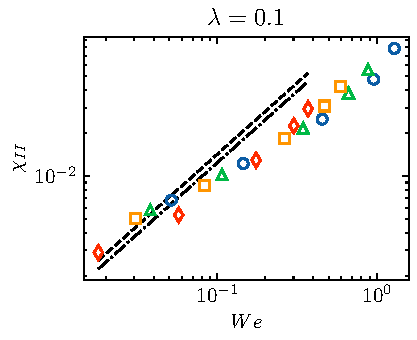
\includegraphics[height = 0.25\textwidth]{image/HOMOGENEOUS_final/PA/chi2_l_1.pdf}
    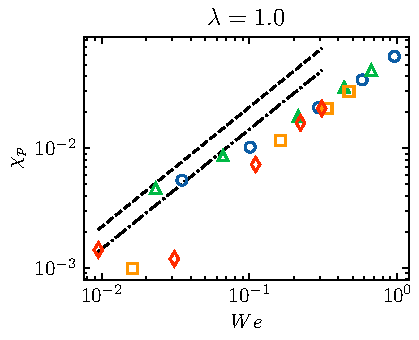
\includegraphics[height = 0.25\textwidth]{image/HOMOGENEOUS_final/PA/chi2_l_10.pdf}
    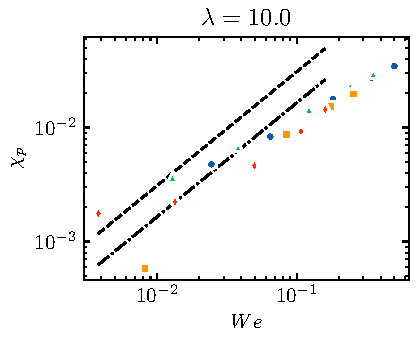
\includegraphics[height = 0.25\textwidth]{image/HOMOGENEOUS_final/PA/chi2_l_100.pdf}
    \caption{
        Mean aspect ratio $\chi_{II}$ (aspect ratio in the direction normal to the flow direction) of the droplets in terms of the \textit{Weber} number based on the mean relative velocity $\textbf{u}_{pf}$. 
        Three viscosity ratio are presented: (left) $\lambda = 0.1$ (middle) $\lambda = 1$ (right) $\lambda = 10$. 
        The density ratio is fixed to $\zeta = 0.9$, and \textit{Bond} number $Bo =0.5$. 
        (symbols) DNS results of $\chi_{II}$ with :
        ($\pmb\bigcirc$) $\phi = 0.01$; ($\pmb\triangle$) $ \phi = 0.05$; ($\pmb\square$) $\phi = 0.1$ ($\pmb\lozenge$) $\phi = 0.2$ with $Bo = 0.5$.
        (dashed line) theoretical formula \ref{eq:deformation_final} supposed valid at $\mathcal{O}(We)$ and $\mathcal{O}(\phi)$. 
        (dot-dashed line) theoretical prediction of \citet{taylor1964deformation}. 
     }
     \label{fig:compare_def_with_DNS}
\end{figure}
It is clear from \ref{fig:compare_def_with_DNS} that the deformation seems to be equally predicted by \citet{taylor1964deformation}'s formula (21), or \ref{eq:deformation_final}. 
Indeed, in \ref{fig:compare_def_with_DNS} the (\textcolor{blue}{$\pmb\bigcirc$}) symbols corresponding to $\phi = 0.01$ are a bit underpredicted by \citet{taylor1964deformation}'s formula for the lowest \textit{Weber} number, while \ref{eq:deformation_final} overpredict a bit the deformation. 
Nevertheless, we can still conclude from \ref{fig:compare_def_with_DNS} that \ref{eq:deformation_final} predicts reasonably well the deformation of the droplet in the expected regime.
Anyhow, both formula differ from a factor of $2$ maximum for $\lambda = 10$ (see \ref{fig:compare_def_with_DNS} (right)). 

Additionally, we can remark that the deformation measured by the DNS results is nearly independent of the volume fraction $\phi$ at fixed $We$, and depends linearly on $We$. 
Therefore, we can conclude that the possible higher order terms in $\phi$ present on the right-hand side of \ref{eq:deformation_final1} are probably negligible and that only the higher order inertial terms matter. 


\subsubsection{First moment of forces}

Now let us turn our attention to the first moment of force calculation. 
The computation of the first moment within DNS requires a surface integral of the stress, specifically the integral of $\textbf{r}\bm\sigma_f^0\cdot\textbf{n}$. 
In our DNS we use VoF method, thus it is quite complicated to implement such an integration directly (although not impossible).
Therefore we compute the first moment of the forces indirectly. 
Indeed, since our simulations are statistically steady and homogeneous, the following balance holds, (see \ref{eq:dt_hybrid_Sp})
\begin{multline}
    \pSavg{\textbf{r}\bm\sigma_f^0\cdot \textbf{n}_d}
    = 
    - \pOavg{\rho_d \textbf{w}_d^0  \textbf{w}_d^0 }\\
    + \pOavg{(-p_d^0 \bm\delta + 2\mu_d \textbf{e}_d^0)}
    +  \pSavg{\gamma (\bm\delta - \textbf{nn})}
\end{multline}
From which we deduce the isotropic and deviatoric part of \ref{eq:stresslet_trans}, namely 
\begin{multline}
    \pSavg{[\textbf{r}\bm\sigma_f^0 - \frac{1}{3}(\textbf{r}\cdot \bm\sigma_f^0)\bm\delta]\cdot \textbf{n}_d}
    - \pOavg{(\mu_f 2 \textbf{e}_d^0  -  p_f\bm\delta)}\\
    = 
    - \pOavg{\rho_d \textbf{w}_d^0  \textbf{w}_d^0 }
    + \pOavg{[-(p_d^0-p_f) \bm\delta + 2(\mu_d-\mu_f) \textbf{e}_d^0]}\\
    + \gamma \pSavg{ (\bm\delta - \textbf{nn})}
    \label{eq:stresslet_dev}
\end{multline}
and, 
\begin{multline}
    \frac{1}{3}\pSavg{\textbf{r}\cdot\bm\sigma_f^0\cdot \textbf{n}_d}
    + \pOavg{p_f}\\
    = 
    -\frac{1}{3} \pOavg{\rho_d \textbf{w}_d^0 \cdot  \textbf{w}_d^0 }
    - \pOavg{(p_d^0-p_f) }
    + \frac{\gamma 2}{3} \intS{},
    \label{eq:stresslet_iso}
\end{multline}
respectively. 
In \ref{eq:stresslet_iso} and \ref{eq:stresslet_dev} only volume integrals are required.
The only exceptions are the last term of \ref{eq:stresslet_dev,eq:stresslet_iso}.
However, these terms are geometrical, i.e. they do not involve dynamical quantities (such as the local stress $\bm\sigma_f^0$) hence it can be computed relatively easily with \texttt{Basilisk}\footnote{In \texttt{Basilisk} we use PLIC method (see \ref{chap:DNS} or \citet{tryggvason2011direct}) to reconstruct the droplets interfaces. 
Therefore, one can easily obtain the normal \textbf{n} and the surface area of the interfaces within each cell of the numerical domain.}.



Based on \ref{eq:stresslet_dev,eq:stresslet_iso} we are then able to compute the values of the whole first moment of force in our DNS and recover the values of the scalar $C_1$ and $C_2$ appearing in \ref{eq:stresslet_trans}. 
As discussed above it is interesting to compare these constants to $- C_2^{Re}$ and $-C_1^{Re}$ as they appear (with opposite sign) in the averaged effective stress \eqref{eq:stress_closed}. 
However, the values of $C_2^{Re}$ and $C_1^{Re}$ presented in \ref{eq:Reynolds_stress} are limited to the low inertial and dilute regime. 
Hence, in this section, we use the values of $C_2^{Re}$ and $C_1^{Re}$ that are directly measured within the DNS (see \ref{chap:pseudoturbulence}). 

On \ref{fig:Sdev_DNS} we display the values of $-C_1$ and $C_1^{Re}$, hence comparing the deviatoric part of the first moment of force and the Reynolds stress tensor, respectively. 
First, it is seen that \ref{eq:stresslet_trans} agrees relatively well with the DNS results in its range of validity ($Re < 1$ and $\phi \ll 1$). 
Surprisingly, we can observe that the $C_1$ measured with the DNS remains approximately constant for all $Re$ and $\phi$ presented here, (except for the case $\lambda = 10$ where larger variations are observed).
We conclude that the stresslet quantity is $\sim Re\phi$ in the whole ranges of parameters presented here. 
Now let us compare the values of $C_1$ and the values of the deviatoric part of the Reynolds stress tensor. 
The first remark is that, as predicted by the theory, both contributions have opposite signs ($C_1 <0$ and $C_1^{Re} > 0$), hence providing both positive contributions to the averaged stress $\bm\sigma_f^\text{eq}$. 
Then, we can observe that $C_1^{Re} \ll C_1$ for the dilute regime ($\phi =0.01$). 
However, as $\phi$ increases $C_1^{Re}$ decreases (because of the $\phi^{-1/3}$ scaling) and therefore in the dense scenarios ($\phi =0.2$) both contributions become comparable.
Particularly, note that for $\lambda = 0.1$, $Re >10$ and $\phi =0.2$ we obtain $2 C_1 \approx  C_1^{Re}$. 
\begin{figure}[h!]
    \centering
    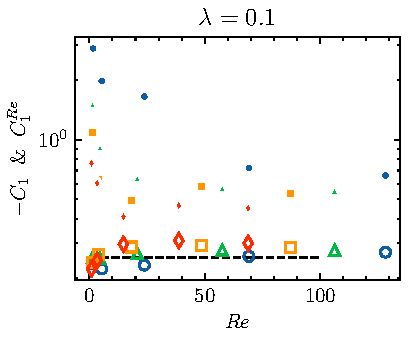
\includegraphics[height = 0.25\textwidth]{image/HOMOGENEOUS_final/PA/Sdev_l_1.pdf}
    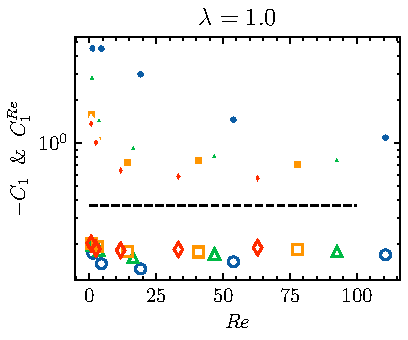
\includegraphics[height = 0.25\textwidth]{image/HOMOGENEOUS_final/PA/Sdev_l_10.pdf}
    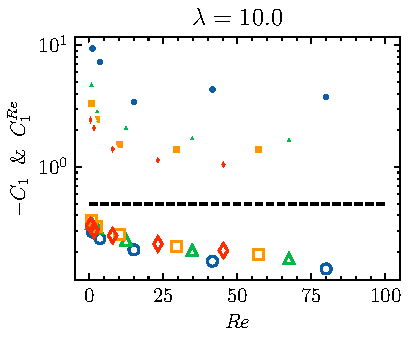
\includegraphics[height = 0.25\textwidth]{image/HOMOGENEOUS_final/PA/Sdev_l_100.pdf}
    \caption{
        Comparison of the coefficients $-C_1$ (hydrodynamic first moment) and $C_1^{Re}$ (Reynolds stress) appearing in \ref{eq:stress_closed} in terms of the \textit{Reynolds} number based on the mean relative velocity $\textbf{u}_{pf}$ for several volume fractions.
        Three viscosity ratio are presented: (left) $\lambda = 0.1$ (middle) $\lambda = 1$ (right) $\lambda = 10$. 
        The density ratio is fixed to $\zeta = 0.9$, and \textit{Bond} number $Bo =0.5$. 
        (Hollow symbols) Mean coefficient $C_1$ measured with the DNS. 
        ($\pmb\bigcirc$) $\phi = 0.01$; ($\pmb\triangle$) $ \phi = 0.05$; ($\pmb\square$) $\phi = 0.1$ ($\pmb\lozenge$) $\phi = 0.2$ with $Bo = 0.5$.
        (dashed line) theoretical formula \ref{eq:stresslet_trans} valid at $\mathcal{O}(Re)$ and $\mathcal{O}(\phi)$. 
        (Filled symbols) Values of the Reynolds stress constant $C_1^{Re}$ for different volume fraction (indicated by the shape of the symbols) based the DNS results \eqref{chap:pseudoturbulence}. 
     }
     \label{fig:Sdev_DNS}
\end{figure}


\begin{figure}[h!]
    \centering
    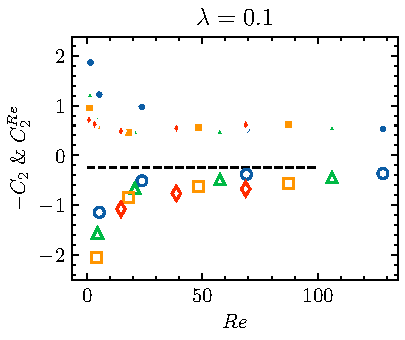
\includegraphics[height = 0.25\textwidth]{image/HOMOGENEOUS_final/PA/Str_l_1.pdf}
    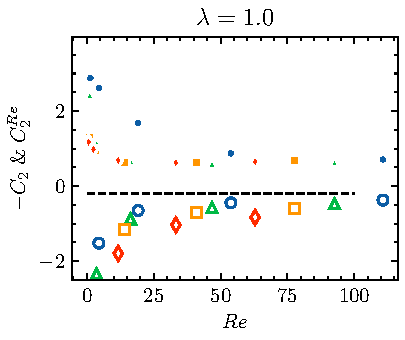
\includegraphics[height = 0.25\textwidth]{image/HOMOGENEOUS_final/PA/Str_l_10.pdf}
    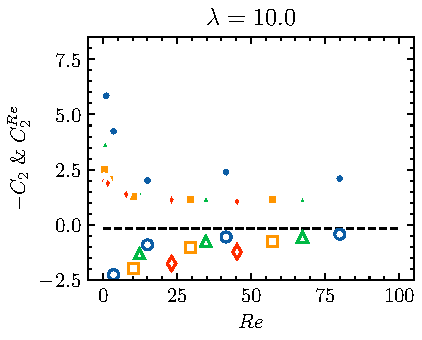
\includegraphics[height = 0.25\textwidth]{image/HOMOGENEOUS_final/PA/Str_l_100.pdf}
    \caption{
        Comparison of the coefficients $-C_2$ and $C_2^{Re}$ appearing in \ref{eq:stress_closed} in terms of the \textit{Reynolds} number based on the mean relative velocity $\textbf{u}_{pf}$ for several volume fractions.
        Three viscosity ratio are presented: (left) $\lambda = 0.1$ (middle) $\lambda = 1$ (right) $\lambda = 10$. 
        The density ratio is fixed to $\zeta = 0.9$, and \textit{Bond} number $Bo =0.5$. 
        (Hollow symbols) Mean coefficient $C_1$ measured with the DNS. 
        ($\pmb\bigcirc$) $\phi = 0.01$; ($\pmb\triangle$) $ \phi = 0.05$; ($\pmb\square$) $\phi = 0.1$ ($\pmb\lozenge$) $\phi = 0.2$ with $Bo = 0.5$.
        (dashed line) theoretical formula \ref{eq:stresslet_trans} valid at $\mathcal{O}(Re)$ and $\mathcal{O}(\phi)$. 
        (Filled symbols) Values of the Reynolds stress constant $C_2^{Re}$ for different volume fraction (indicated by the shape of the symbols) based the DNS results \eqref{chap:pseudoturbulence}. 
     }
     \label{fig:Str_DNS}
\end{figure}
Let us turn our attention to the isotropic part of the Reynolds stress and first moment of the forces, i.e. $C_2$ and $C_2^{Re}$, respectively. 
On \ref{fig:Str_DNS} it is observed that \ref{eq:stresslet_trans} also provides a good estimation for $C_2$. 
Note that \ref{eq:stresslet_trans} seems more accurate for large $Re$ and large $\phi$ than lower ones.
This result is partially fortuitous as we recall that  \ref{eq:stresslet_trans} is only accurate at $\mathcal{O}(Re,\phi)$. 
In opposition to the preceding case note that $ - C_2<0$ and $C_2^{Re} > 0$.  
Hence, the effect of the first moment tends to cancel the contribution of the Reynolds stress in the mean equivalent stress (as predicted by the theory\eqref{eq:stresslet_trans}). 
This last fact becomes even more relevant for large values of $\phi$ where both contributions are comparable in magnitude. 

\section{Conclusion}
This chapter has been divided into two main sections. 
The first presents the results of the closure terms in dilute Stokes flows for spherical droplets. 
The second section focus on the effect of finite Reynolds number on the droplets shape and suspension stress. 
Let us highlight the key advancements:
\begin{enumerate}
    % \item We generalized the work of \citet{zhang1994ensemble} by demonstrating how to relate various ensemble-averaged quantities of the hybrid model, i.e., $\avg{\chi_f\ldots}$, $\pOavg{\ldots}$, and $\pSavg{\ldots}$, to single-particle conditionally averaged quantities. 
    % Furthermore, we provided a concise methodology to derive the single-particle conditionally averaged Navier-Stokes equations without any assumptions on the flow regime, thereby extending the work of \citet{hinch1977averaged}. 
    % \item The rigorous derivation presented in the first sections leads us to a novel decomposition of the interphase momentum exchange term, $\avg{\delta_\Gamma \bm\sigma_f^0 \cdot \textbf{n}}$. 
    % We demonstrated that the classical partition of the drag force term using the mean continuous-phase stress $\bm\sigma_f$ is not the most practical, due to the inclusion of particle contributions within $\bm\sigma_f$.
    % While this partition is not incorrect, it necessitates subtracting $\avg{\delta_\Gamma (\textbf{n}_d \textbf{u}_f' + \textbf{u}_f' \textbf{n}_d)}$ from the integral of the local stress over the particles' surface, when computing the closure term. 
    % It appears that this step is overlooked in numerical studies, as in \citet{wang2021numerical,wang2024effect} where they use this decomposition, leading to an inconsistent formulation between the drag force term and what is actually computed.
    % Instead of $\bm\sigma_f$, we propose to use what we called the mean Newtonian stress: $\bm\Sigma_f = -p_f \bm\delta + \mu_f [\grad \textbf{u}_f + (\grad \textbf{u}_f)^\dagger]$. 
    % \item Using distribution theory, we re-derived equation (2.10) from \citet{batchelor1972sedimentation}, which establishes the link between ensemble-averaged continuous-phase quantities $\avg{\chi_f\ldots}$ and the single-particle conditioned averaged quantity $f_f^1$. 
    % Our approach provided an explicit expression for the error terms introduced during the derivation of this formula.
    % We showed that instead of the predicted $\mathcal{O}(\phi_d^2)$ error from \citet{batchelor1972sedimentation}, the actual error scales as $\mathcal{O}(f_f^1 r)$, where $r$ is the distance from the particle's center of mass. 
    % This is a significant advancement because it explains why equation (2.10) diverges for certain functions $f_f^1$: the error in such cases becomes infinite, making the formula unphysical.
    % We also demonstrated that in an inhomogeneous flow (which is always the case in practical application), the equivalent of (2.10) of \citet{batchelor1972sedimentation} for inhomogeneous flows always results in a divergent integral, for any physical function $f_f^1$.
    % \item Then it is shown that the \textit{Conditionally averaged quantities} obey the \textit{single-particle conditionally} averaged equations which are derived assumption-free. 
    % We demonstrated how the boundary conditions of the \textit{Conditionally averaged quantities} make the bridge between the closure problem and the ensemble-averaged quantities. 
    % Notably, complex features of the flow, such as gradient of volume fraction, and background velocity gradient, can be taken into account through the boundary conditions of $\phi^1_d$ and $\textbf{u}^1$. 
    \item Based on the solution for spherical droplets immersed in general linear flow, we derived most of the closures present in the hybrid model. 
    While many of these were already established, we introduced several new closures specifically: 
    the pseudo-turbulent stress $\avg{\chi_f \textbf{u}_f'\textbf{u}_f'}$ generated by a mean shear flow $\textbf{E}_f$ on droplets; 
    The pseudo-turbulent kinetic energy transfer resulting from the local work on the particles surfaces; 
    The continuous phase droplets induced dissipation $\avg{\chi_f \bm\sigma_f^0:\grad \textbf{u}_f^0}$; 
    The averaged droplet internal viscous dissipation term. 
    \item %Finally, we propose an analysis of the impact of the phases relative motion on the particle deformation. % and carrier fluid phase effective stress. 
    We demonstrated an alternative derivation (compared to the study of \citet{taylor1964deformation}) of the droplet deformation generated by relative translation at finite Reynolds number. 
    Our methodology is based on the averaged particle equations derived in \ref{chap:deformable} and explicit closures are derived using the reciprocal theorem suited for spherical droplets (see \ref{ap:reciprocal} for more information). 
    We then compare our results to the DNS results, good agreements are obtained. 
    \item 
    Lastly, we discuss the impact of particle translation on the suspension stress. 
    It is shown that the exchange terms responsible for the droplets deformation, i.e. the \textit{Stresslet} term, is also responsible for an additional source in the continuous phase stress. 
    Notably, we show that the \textit{Stresslet} term usually neglected in this context is not null for small but finite inertial effect and is function of the particle-carrier phase relative velocity square and $\phi Re$.  
    When considering only relative translation this term is in competition with the \textit{Reynolds stress} term, which is shown to be comparable to the \textit{Stresslet} term. 
    As the Reynolds stress term is shown to be $\sim \phi^{2/3}$ while the \textit{Stresslet} is $\sim \phi$ we might expect the latter negligible in the dilute regime but dominant in the dense regime. 
    At $\phi = 0.05$ we state that the contribution of the \textit{Stresslet} is about 10\% of the \textit{Reynolds stress} contribution. 
    We then confirmed with the DNS results that the \textit{Stresslet} approximately reaches the \textit{Reynolds stress} term for high volume fractions ($\phi=0.2$). 
\end{enumerate}
% In summary, more work is needed to provide accurate closure for the first moment of forces that must be included in the averaged models. 